\chapter{系统主要功能与技术细节}
\label{cha:sys}

\section{平台技术架构}

预后模型一体化系统使用的主要技术栈组织结构如图\ref{fig:tech_stk_org}所示:

\begin{figure}[!htbp]
    \centering
    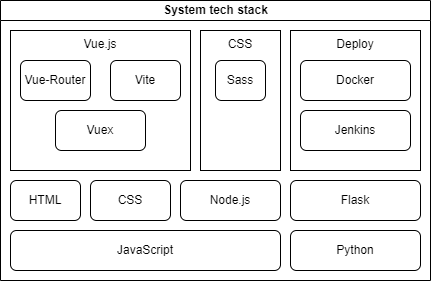
\includegraphics[scale=0.8]{tech_stk_org.drawio.png}
    \caption{系统技术栈组织结构图} \label{fig:tech_stk_org}
\end{figure}

在图中可以看到,系统使用的技术主要基于JS和Python两种语言,这是考虑到模型训练与后端一体化集成的结果。

在前端部分,代码使用的主要架构是Vue.js,组件化的组织模式让代码更有结构性,并使用Vite作为构建工具让开发的过程中编译更加迅速,这让开发的过程大大加快了。同时,考虑到分页需求,需要有不同的页面来展示数据、训练、预测等功能,Vue-Router的引入让选择性渲染和路由管理更加便捷。而相比于单纯的CSS样式表,使用Sass减少了样式的重复,让组件样式更有可重用性。

后端中,本文考虑到模型的训练和预测都在Python中实现,如果使用其他语言会增加代码的复杂度,需要使用文件系统或语言桥进行结合,这大大增加了系统的复杂度和不稳定性。所以为了让代码更健壮,这里使用基于Python的Flask进行开发。同时为了让部署更加便捷,这里使用了Jenkins让部署自动化,只需上传到GitHub就能进行自动部署到服务器的进程,而Docker则让环境更加稳定,不需要通过一系列的脚本进行控制,也不会受到服务器本身环境的桎梏。

\section{页面总体设计}

主要功能页面如图\ref{fig:pages_design}所示:

\begin{figure}[!htbp]
    \centering
    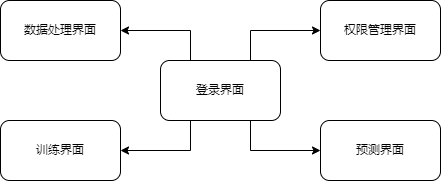
\includegraphics[scale=0.8]{front_end_design.drawio.png}
    \caption{系统页面设计图} \label{fig:pages_design}
\end{figure}

考虑到系统使用需求,需要一个登录页面对用户进行管控,同时也需要设计权限管理功能来让医院管理员对医生进行页面权限管控。而数据页面提供了数据的采集、批量导入、批量导出功能。训练预测界面作为主要功能页面,分别提供了模型训练功能和患者预测功能。其中训练界面可以直接进行文件上传,训练得到的文件被存储在后端中,预测界面中可以使用训练得到的模型文件进行预测,预测结果同时使用一张表进行存储。

\section{后端接口设计}

考虑到系统的需要,首先需要提供账号管理和权限管理相应的接口,考虑到实现内容较为通用,所以这里只提及主要功能相关接口的实现,文件上传、导出相关接口同理。

按照上述页面需求,用户需要对数据页面进行添加和查询,所以对于数据页面需要设计以下接口:

\begin{enumerate}
    \item [1.] 数据列表分页:提供数据的查询功能
    \item [2.] 添加数据请求:输入训练数据
    \item [3.] 删除数据请求:删除训练数据
\end{enumerate}

对于训练页面,需要使用一张表对训练得到的模型文件进行整理,所以接口如下:

\begin{enumerate}
    \item [1.] 训练数据列表分页:提供训练数据的查询功能
    \item [2.] 训练模型请求:输入训练数据集,并集成训练,完成后在模型表中记录
    \item [3.] 删除模型请求:将结果较差或重复的模型删除
\end{enumerate}

对于预测页面,获取模型列表可以直接使用训练页面中的列表并进行裁剪到选择表单中,所以不需要提供额外的接口,只需要提供预测表的分页、添加、删除接口即可:

\begin{enumerate}
    \item [1.] 预测结果列表分页:提供预测结果表的查询功能
    \item [2.] 添加结果请求:集成预测功能,在结果表中记录
    \item [3.] 删除结果请求:将误操作或较差的结果删除
\end{enumerate}

\section{系统部署与测试}

系统的部署使用了阿里云服务器进行测试,在购买服务器后在Jenkins中填入管理账号密码和服务器信息,同时将该服务链接到GitHub仓库中,由于使用了Dokcer进行封装,所以不需要安装很多插件即可使用,最后添加API Token进行验证即可。

同时,后端同样尝试了使用树莓派4B进行人工部署,服务在raspbian系统下局域网中运行情况良好,由于模型需要的性能要求不高,在有一定条件的arm开发板中都可以部署。

\section{系统效果一览}

\begin{figure}[!htbp]
    \centering
    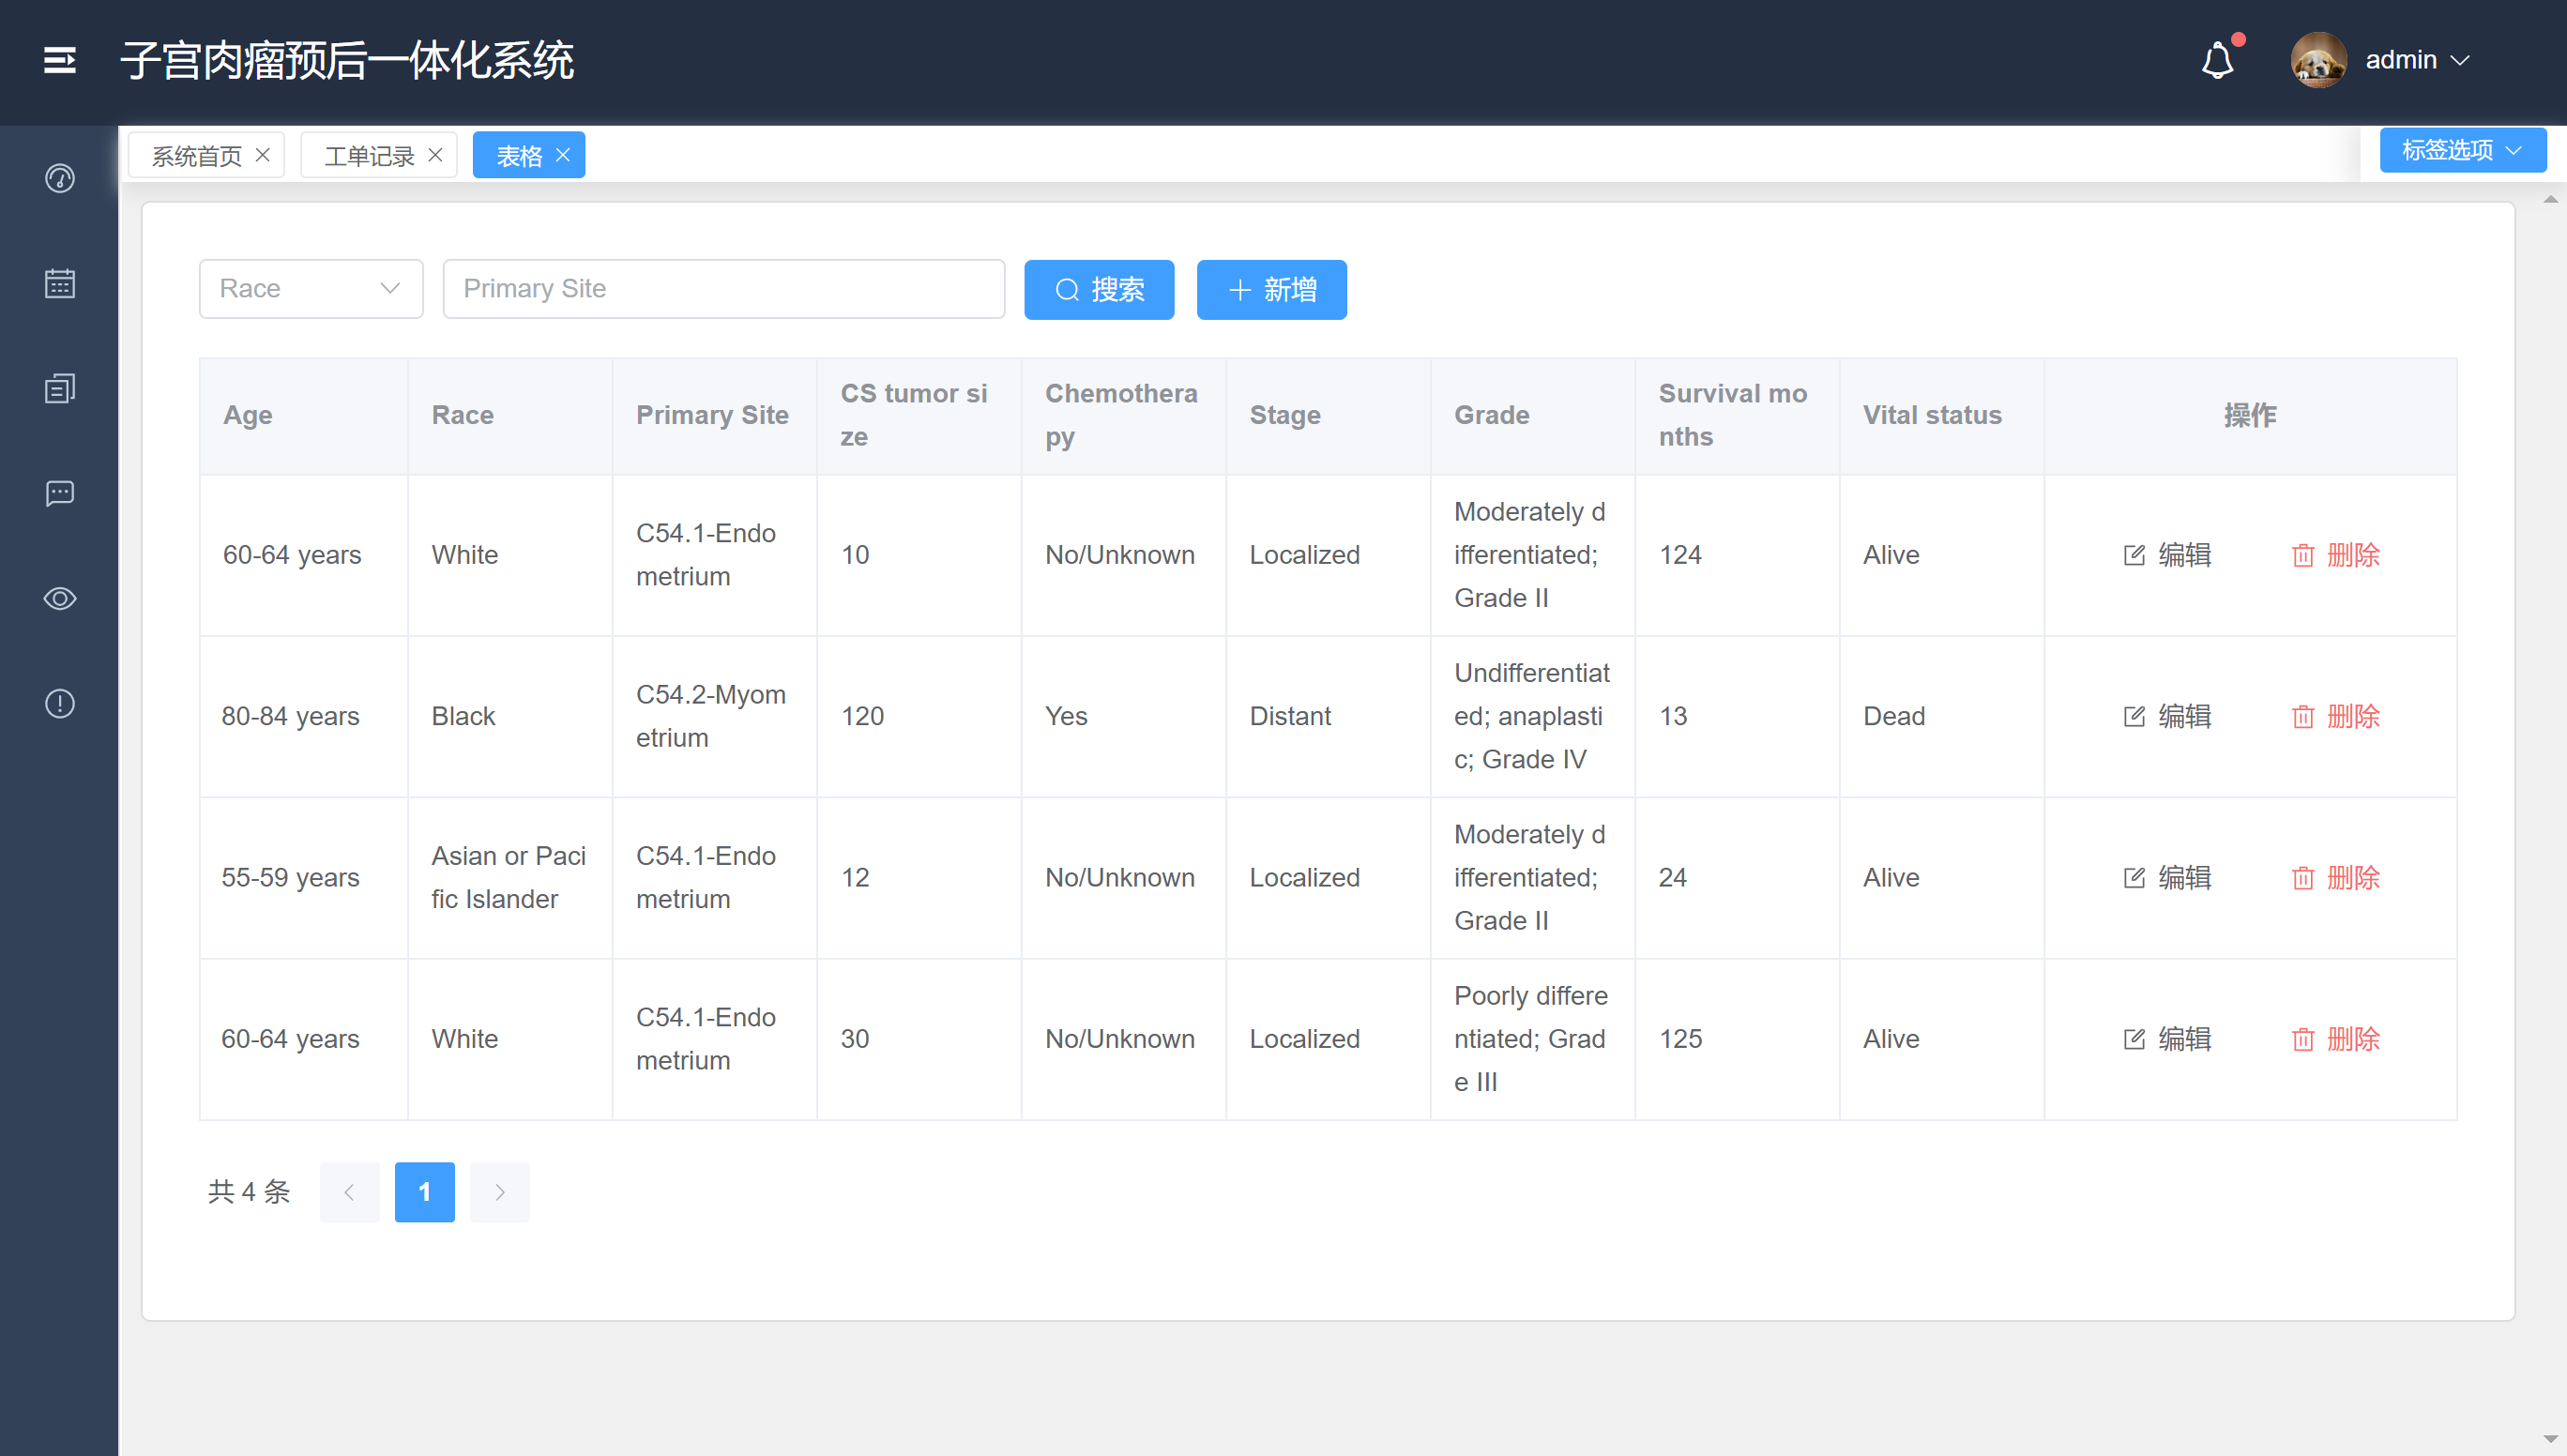
\includegraphics[scale=0.2]{page_table.png}
    \caption{系统表格处理页面} \label{fig:page_table}
\end{figure}

\begin{figure}[!htbp]
    \centering
    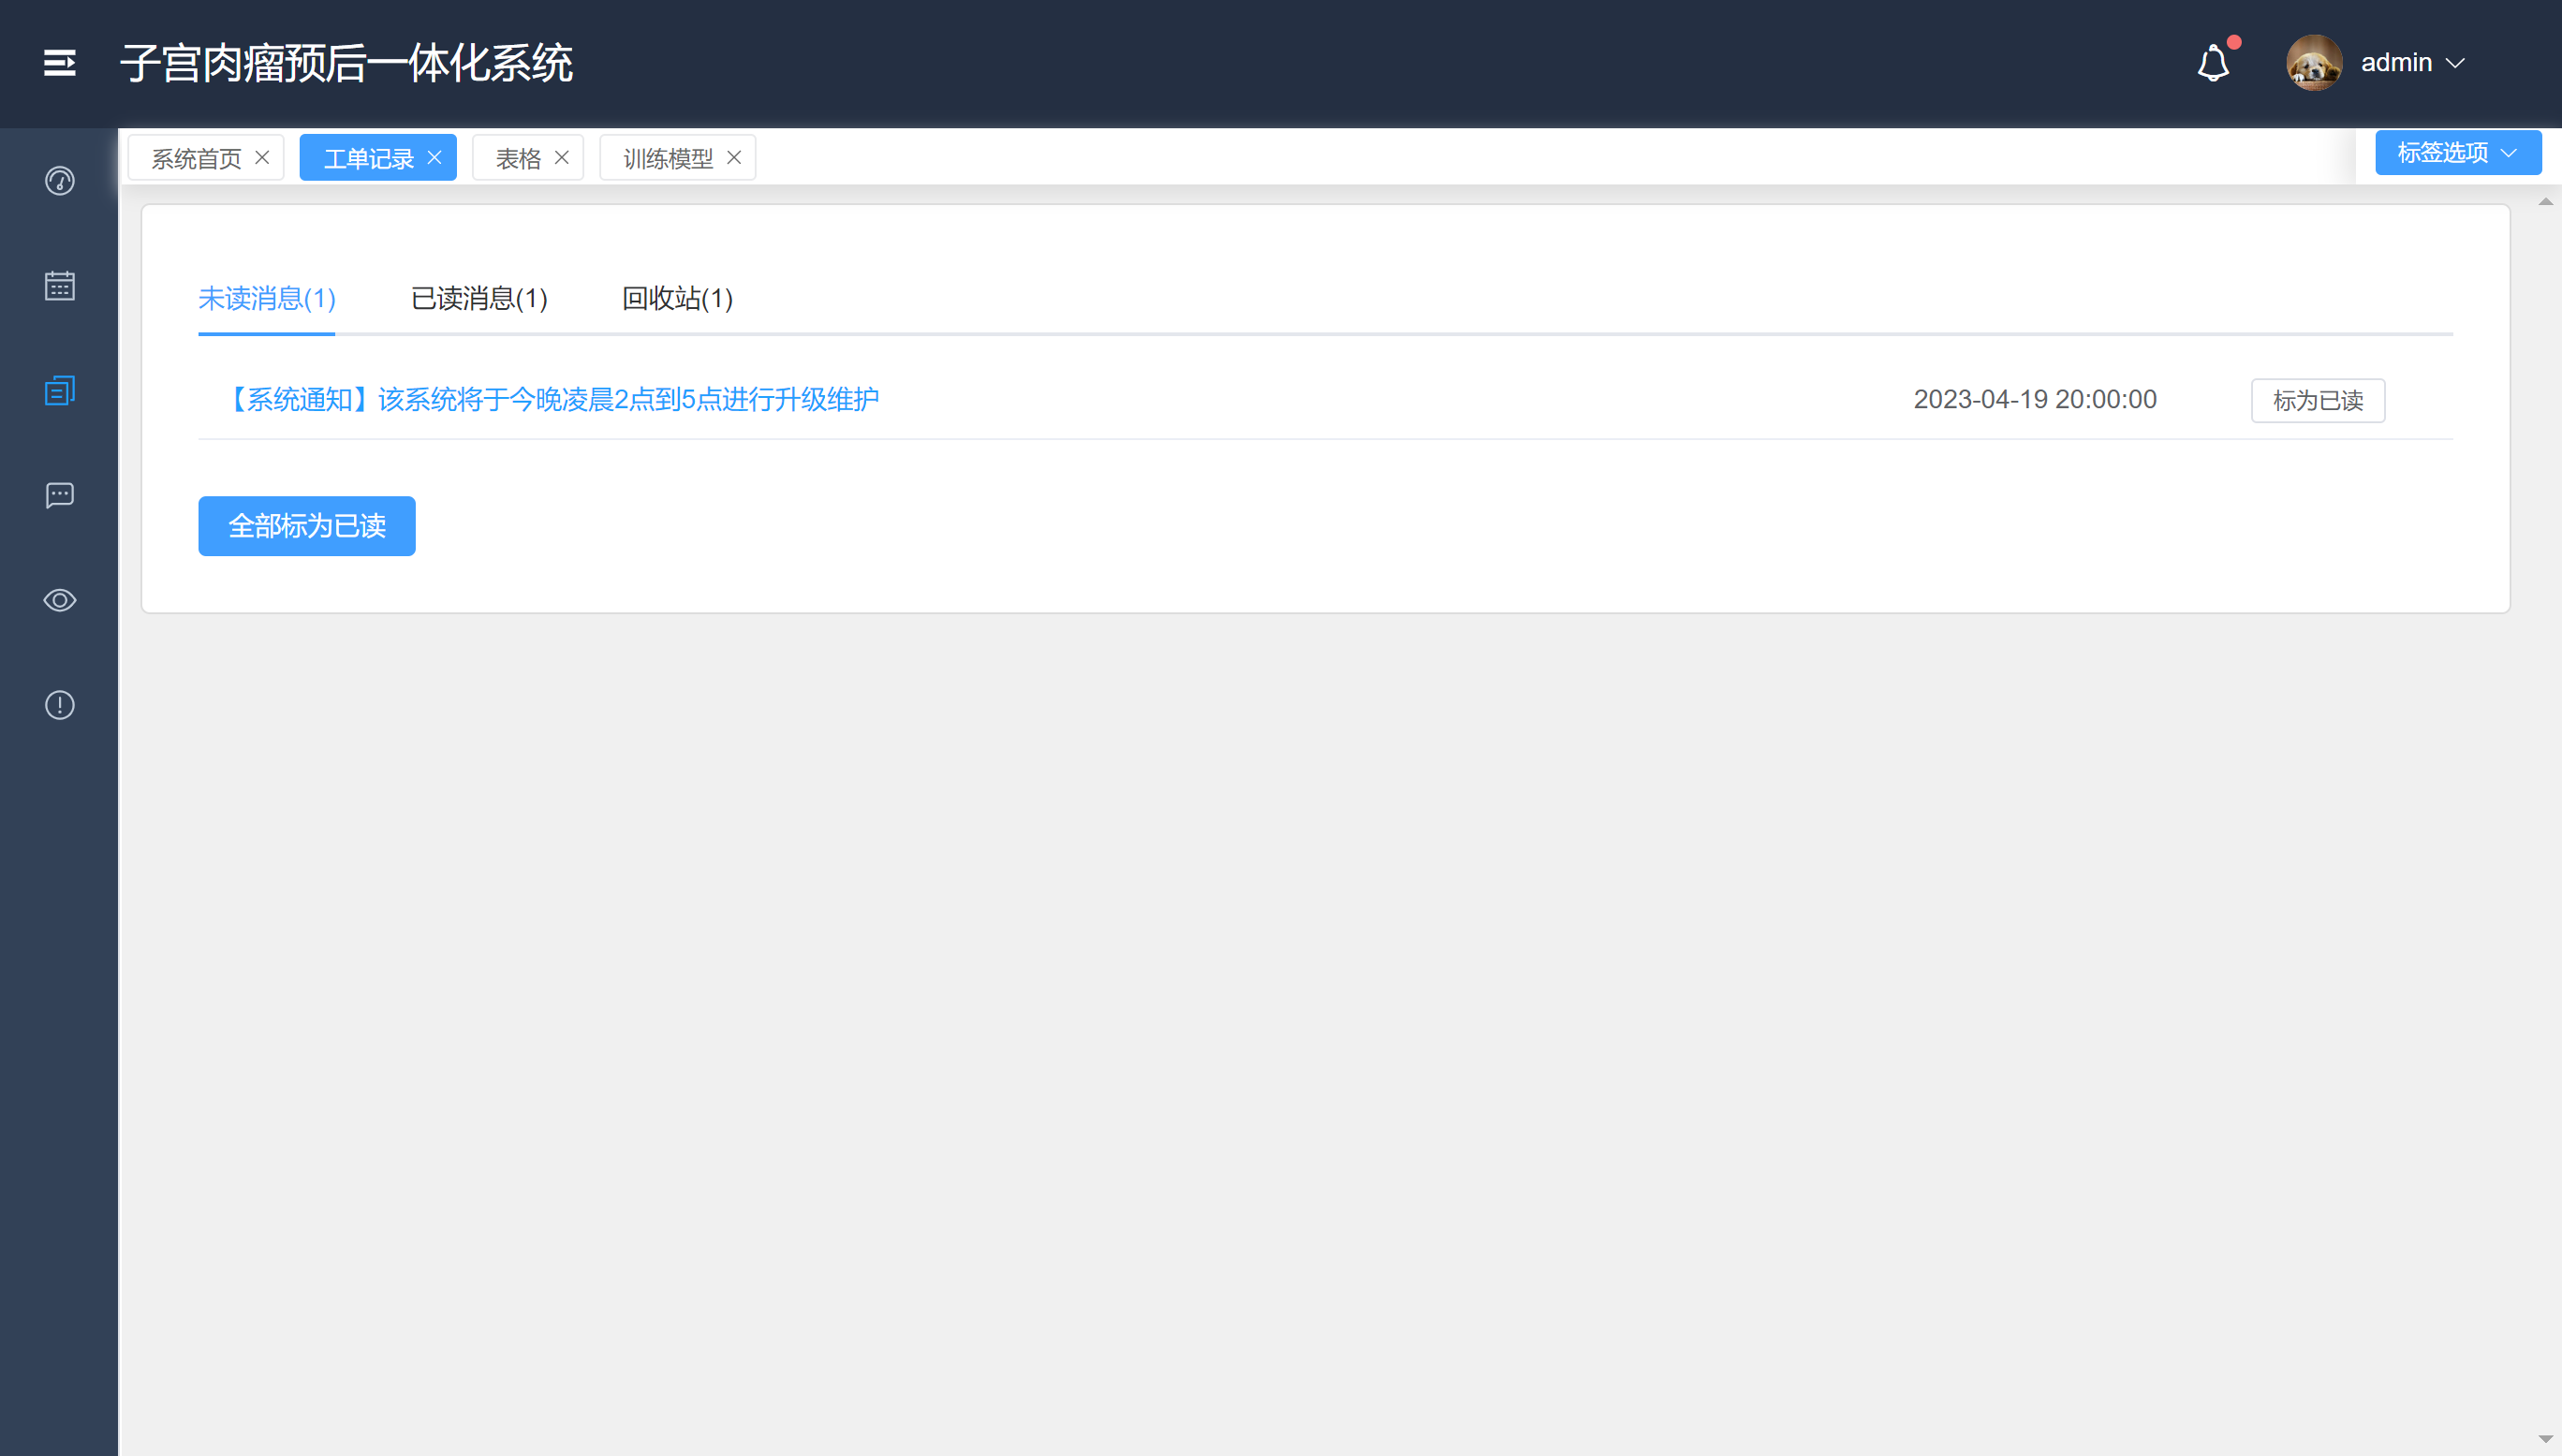
\includegraphics[scale=0.2]{page_msg.png}
    \caption{系统工单页面} \label{fig:page_msg}
\end{figure}

\begin{figure}[!htbp]
    \centering
    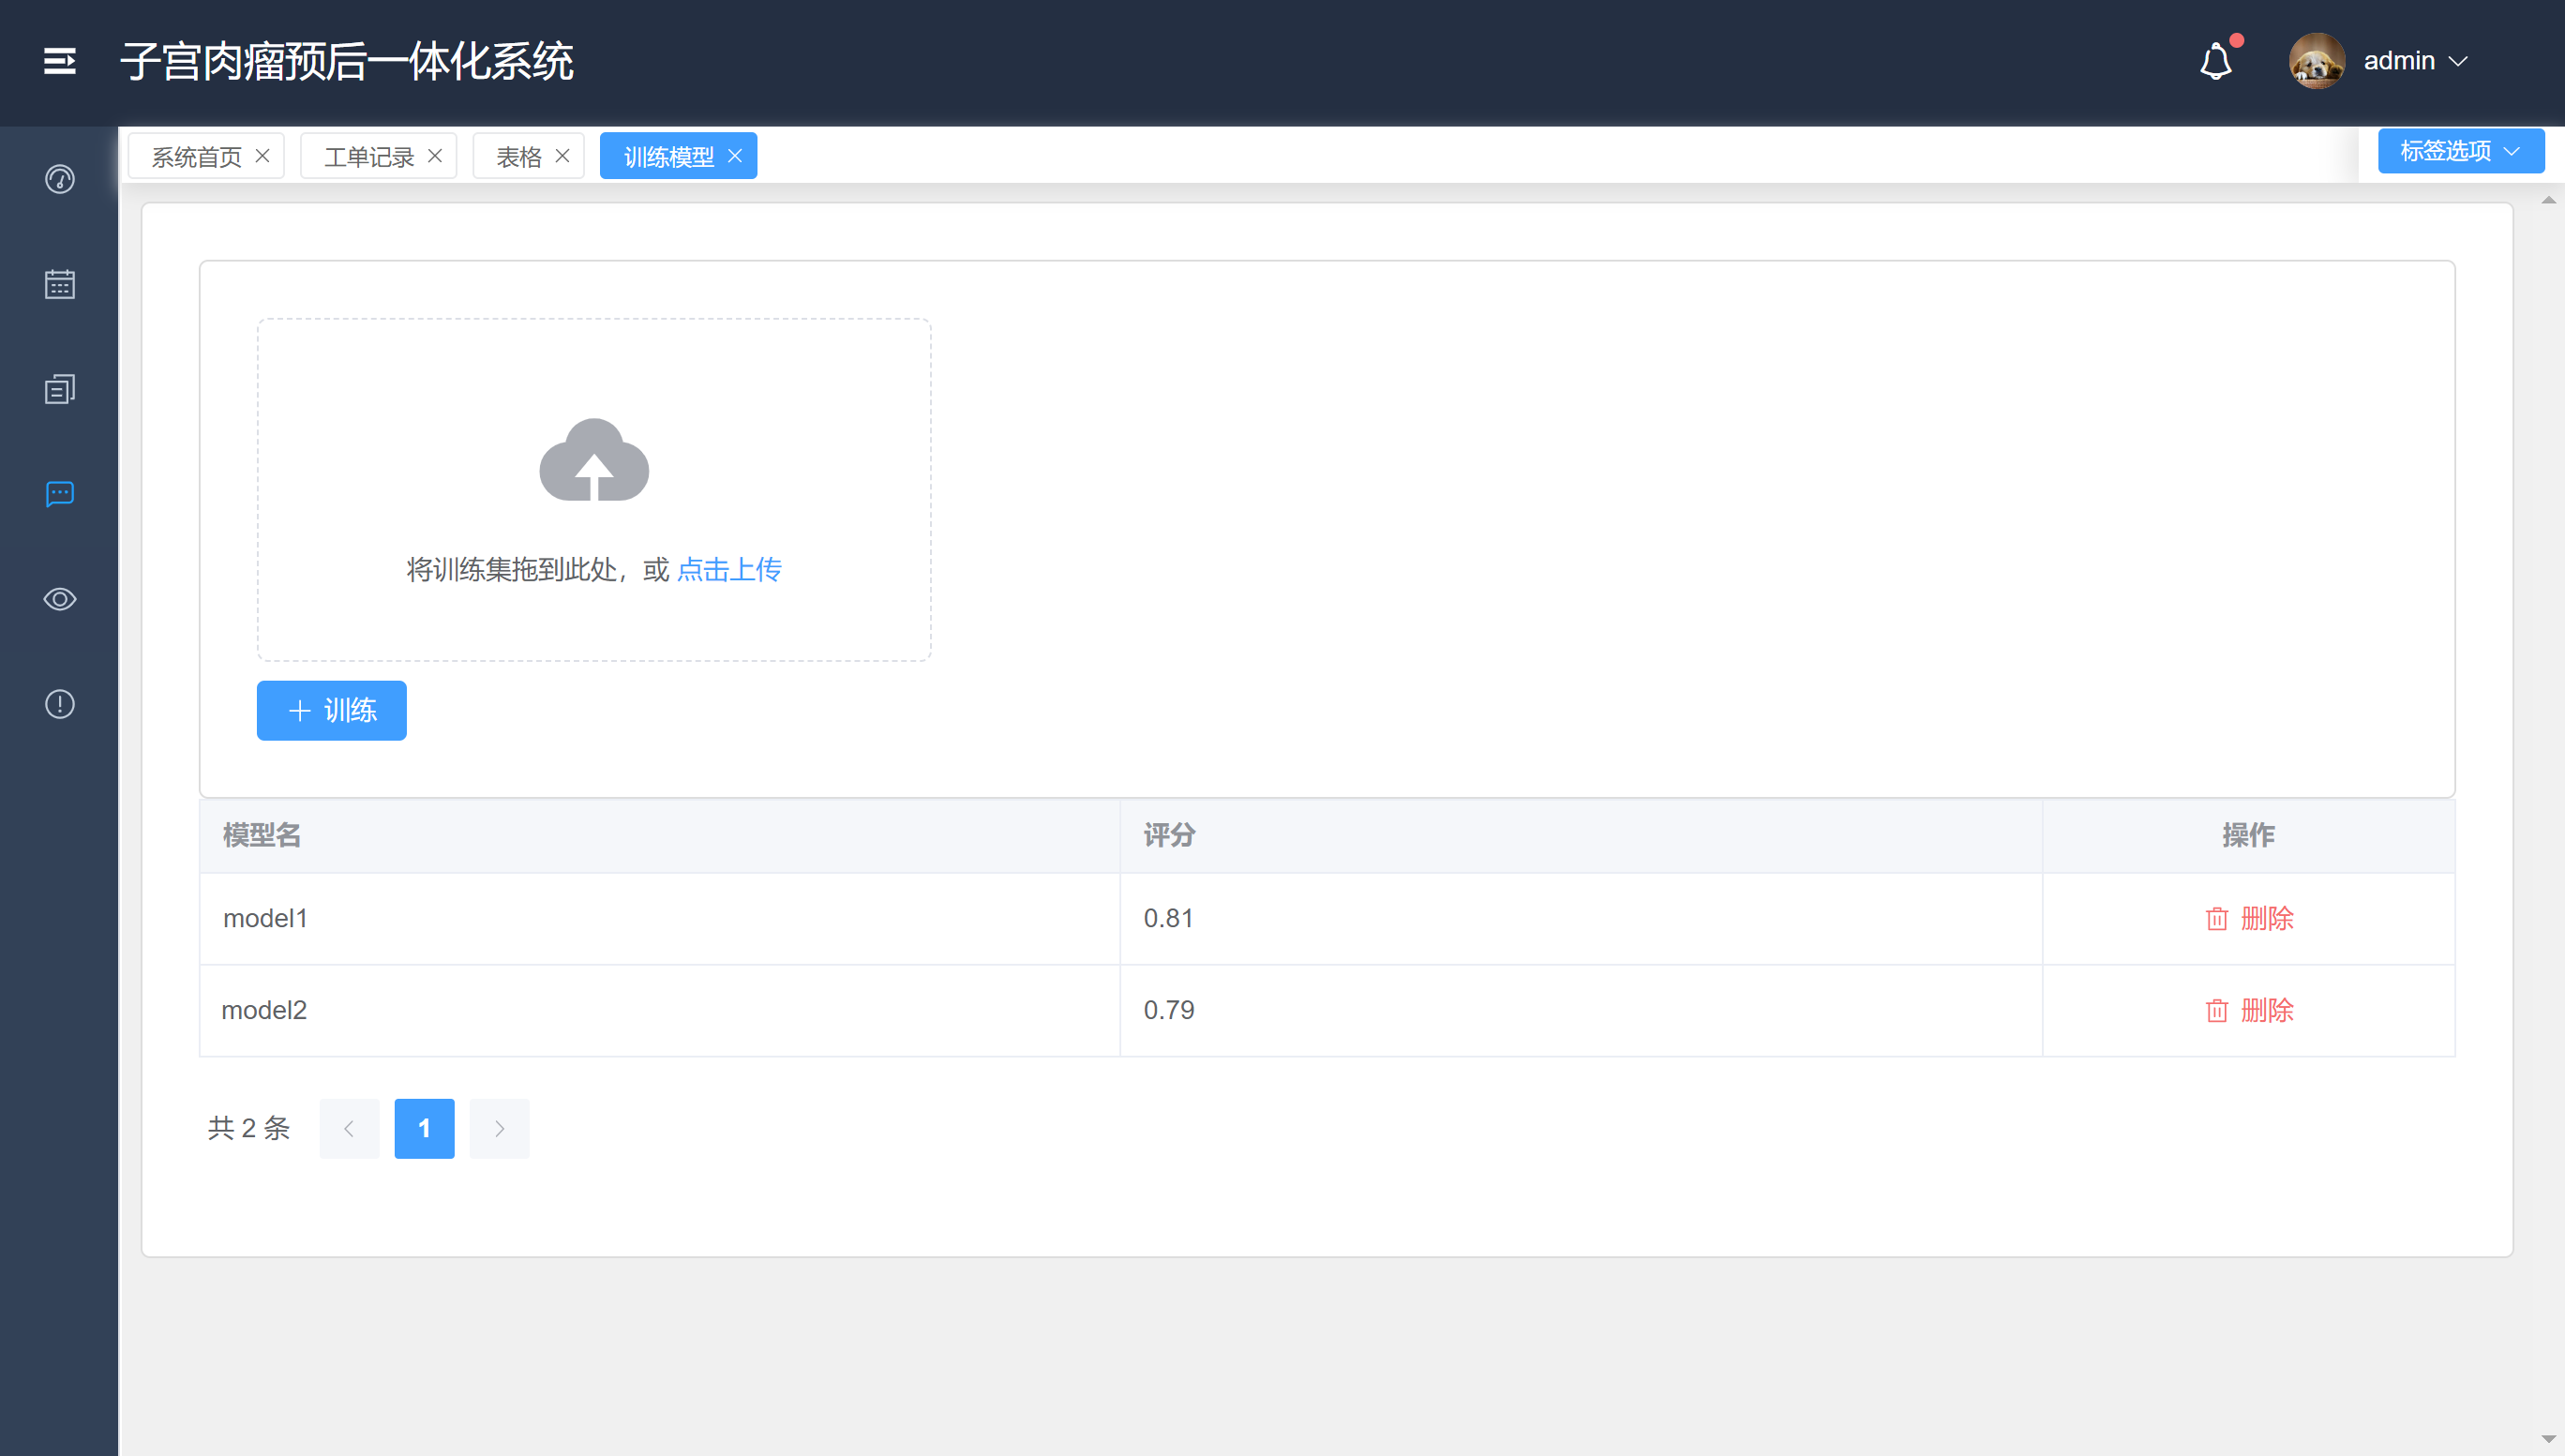
\includegraphics[scale=0.2]{page_train.png}
    \caption{系统训练页面} \label{fig:page_train}
\end{figure}

\begin{figure}[!htbp]
    \centering
    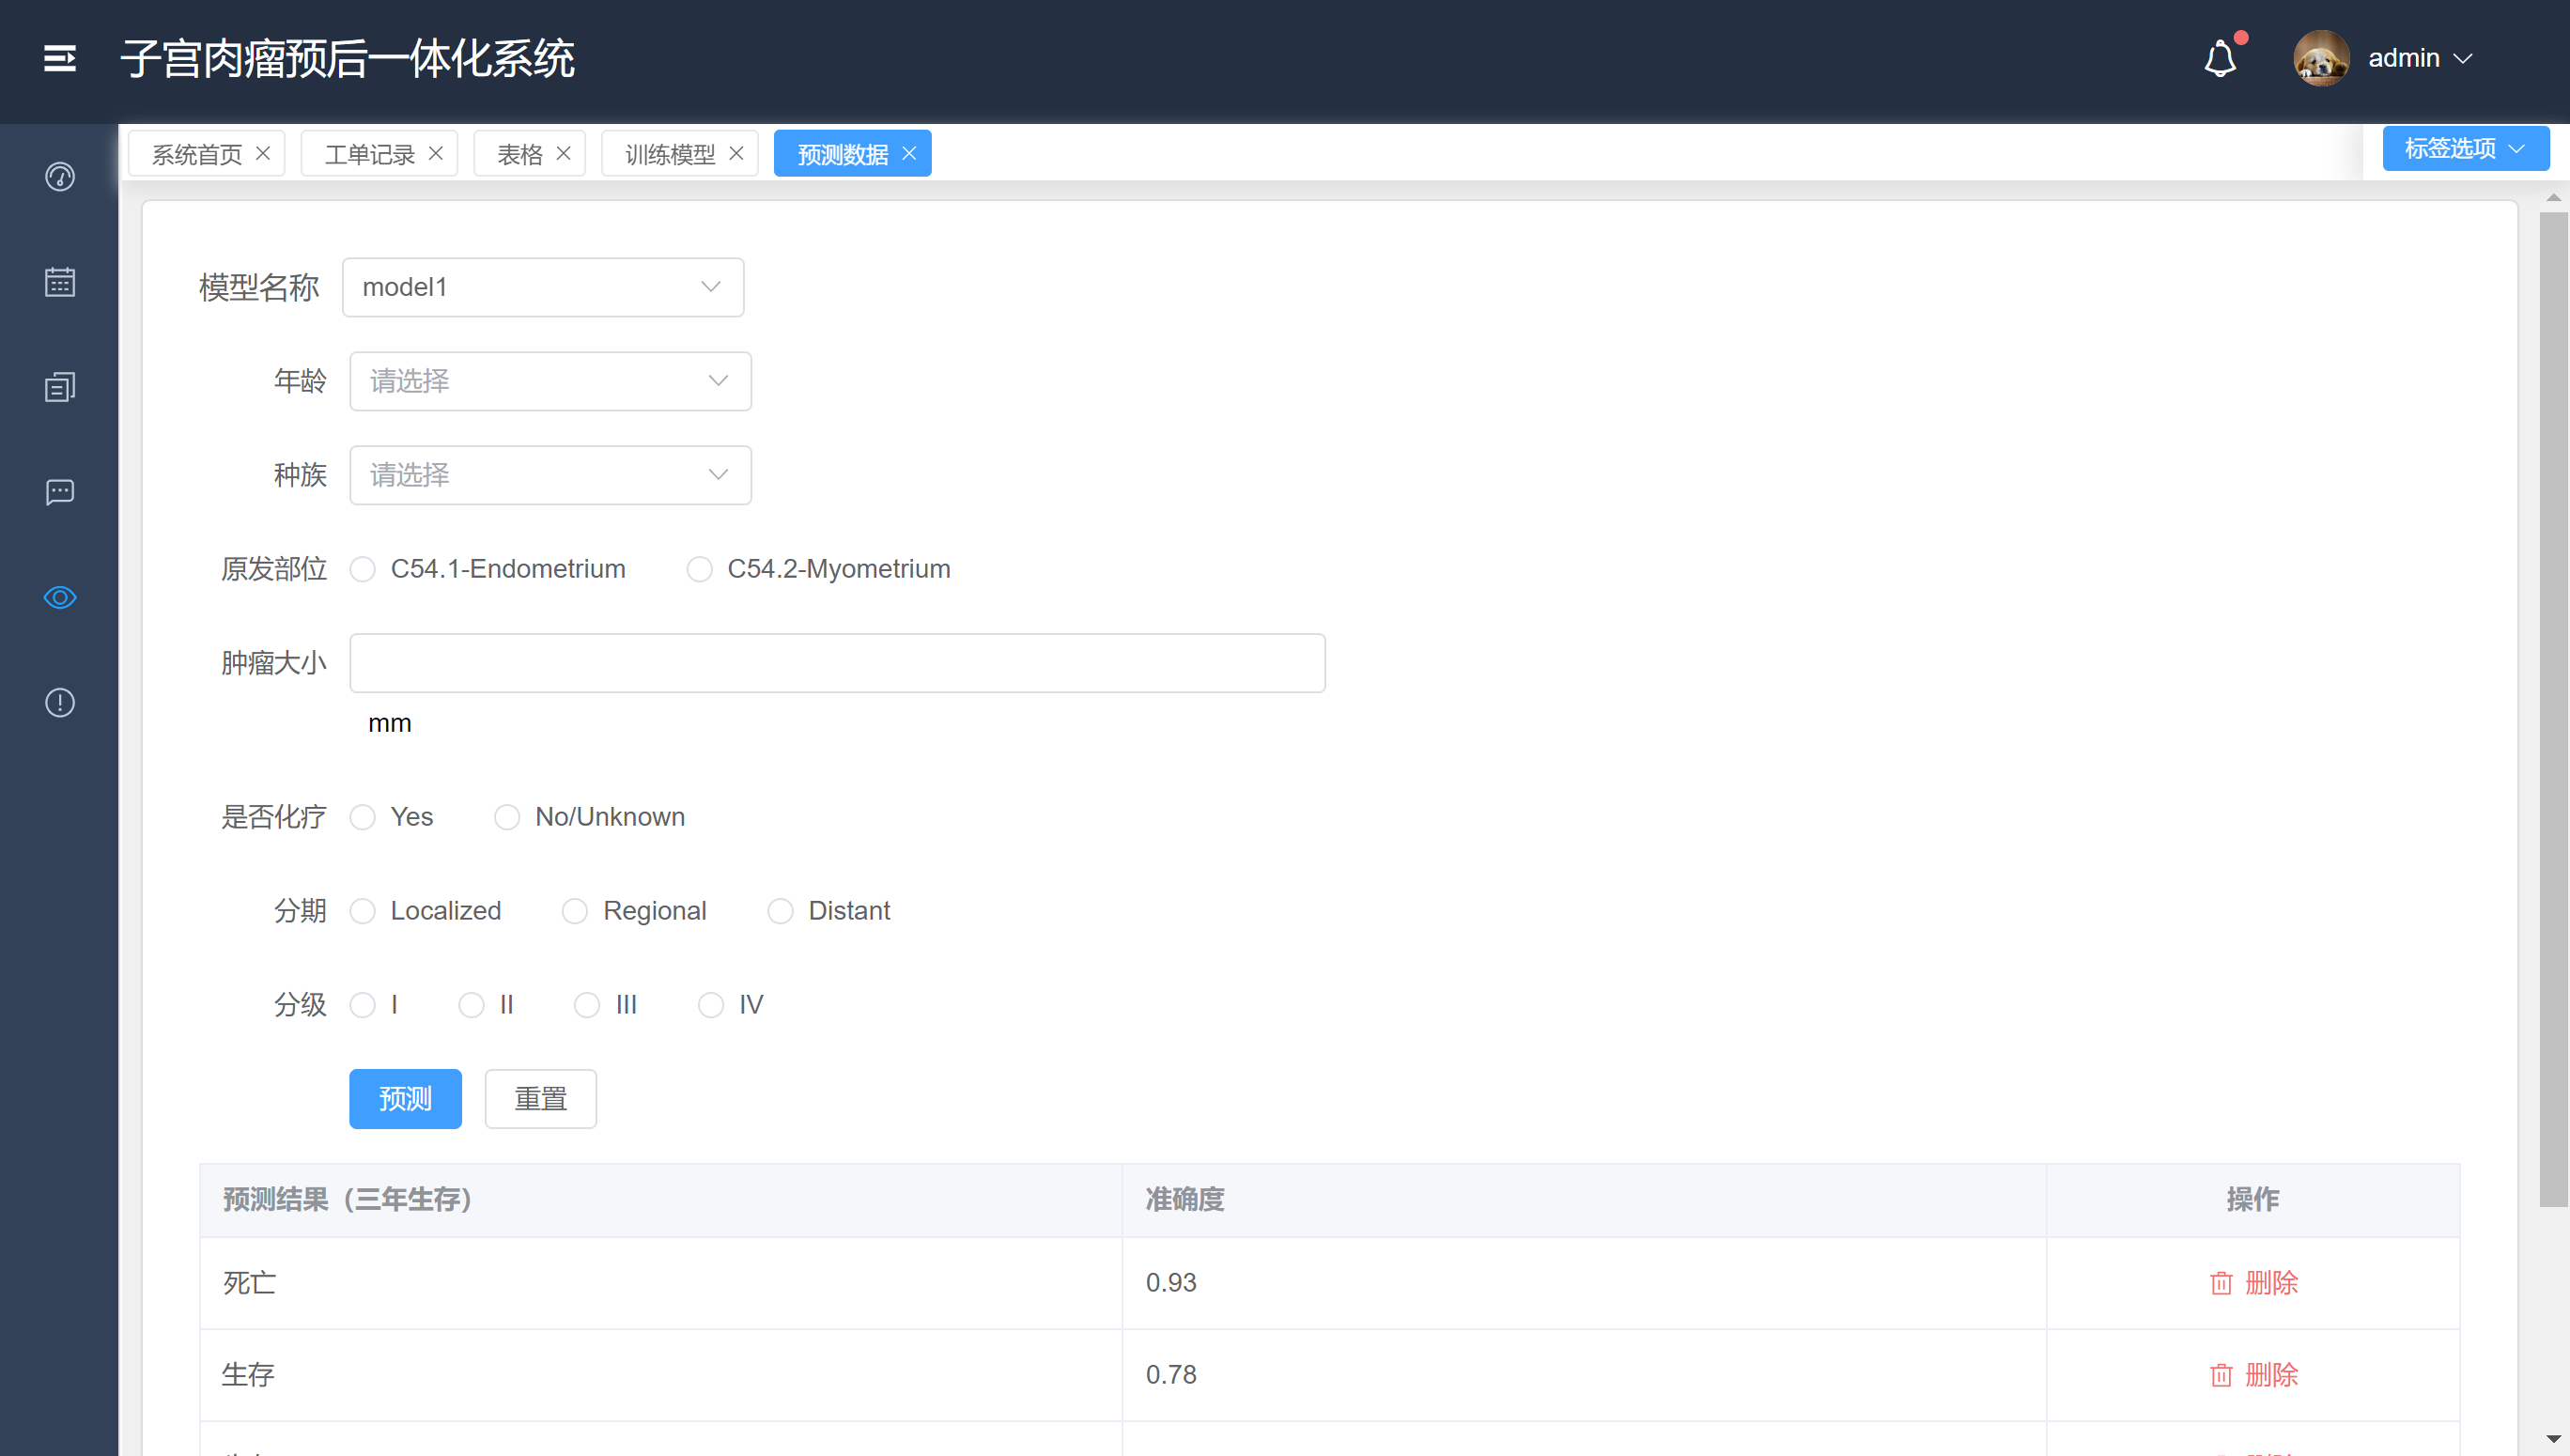
\includegraphics[scale=0.2]{page_pred.png}
    \caption{系统预测页面} \label{fig:page_pred}
\end{figure}

\begin{figure}[!htbp]
    \centering
    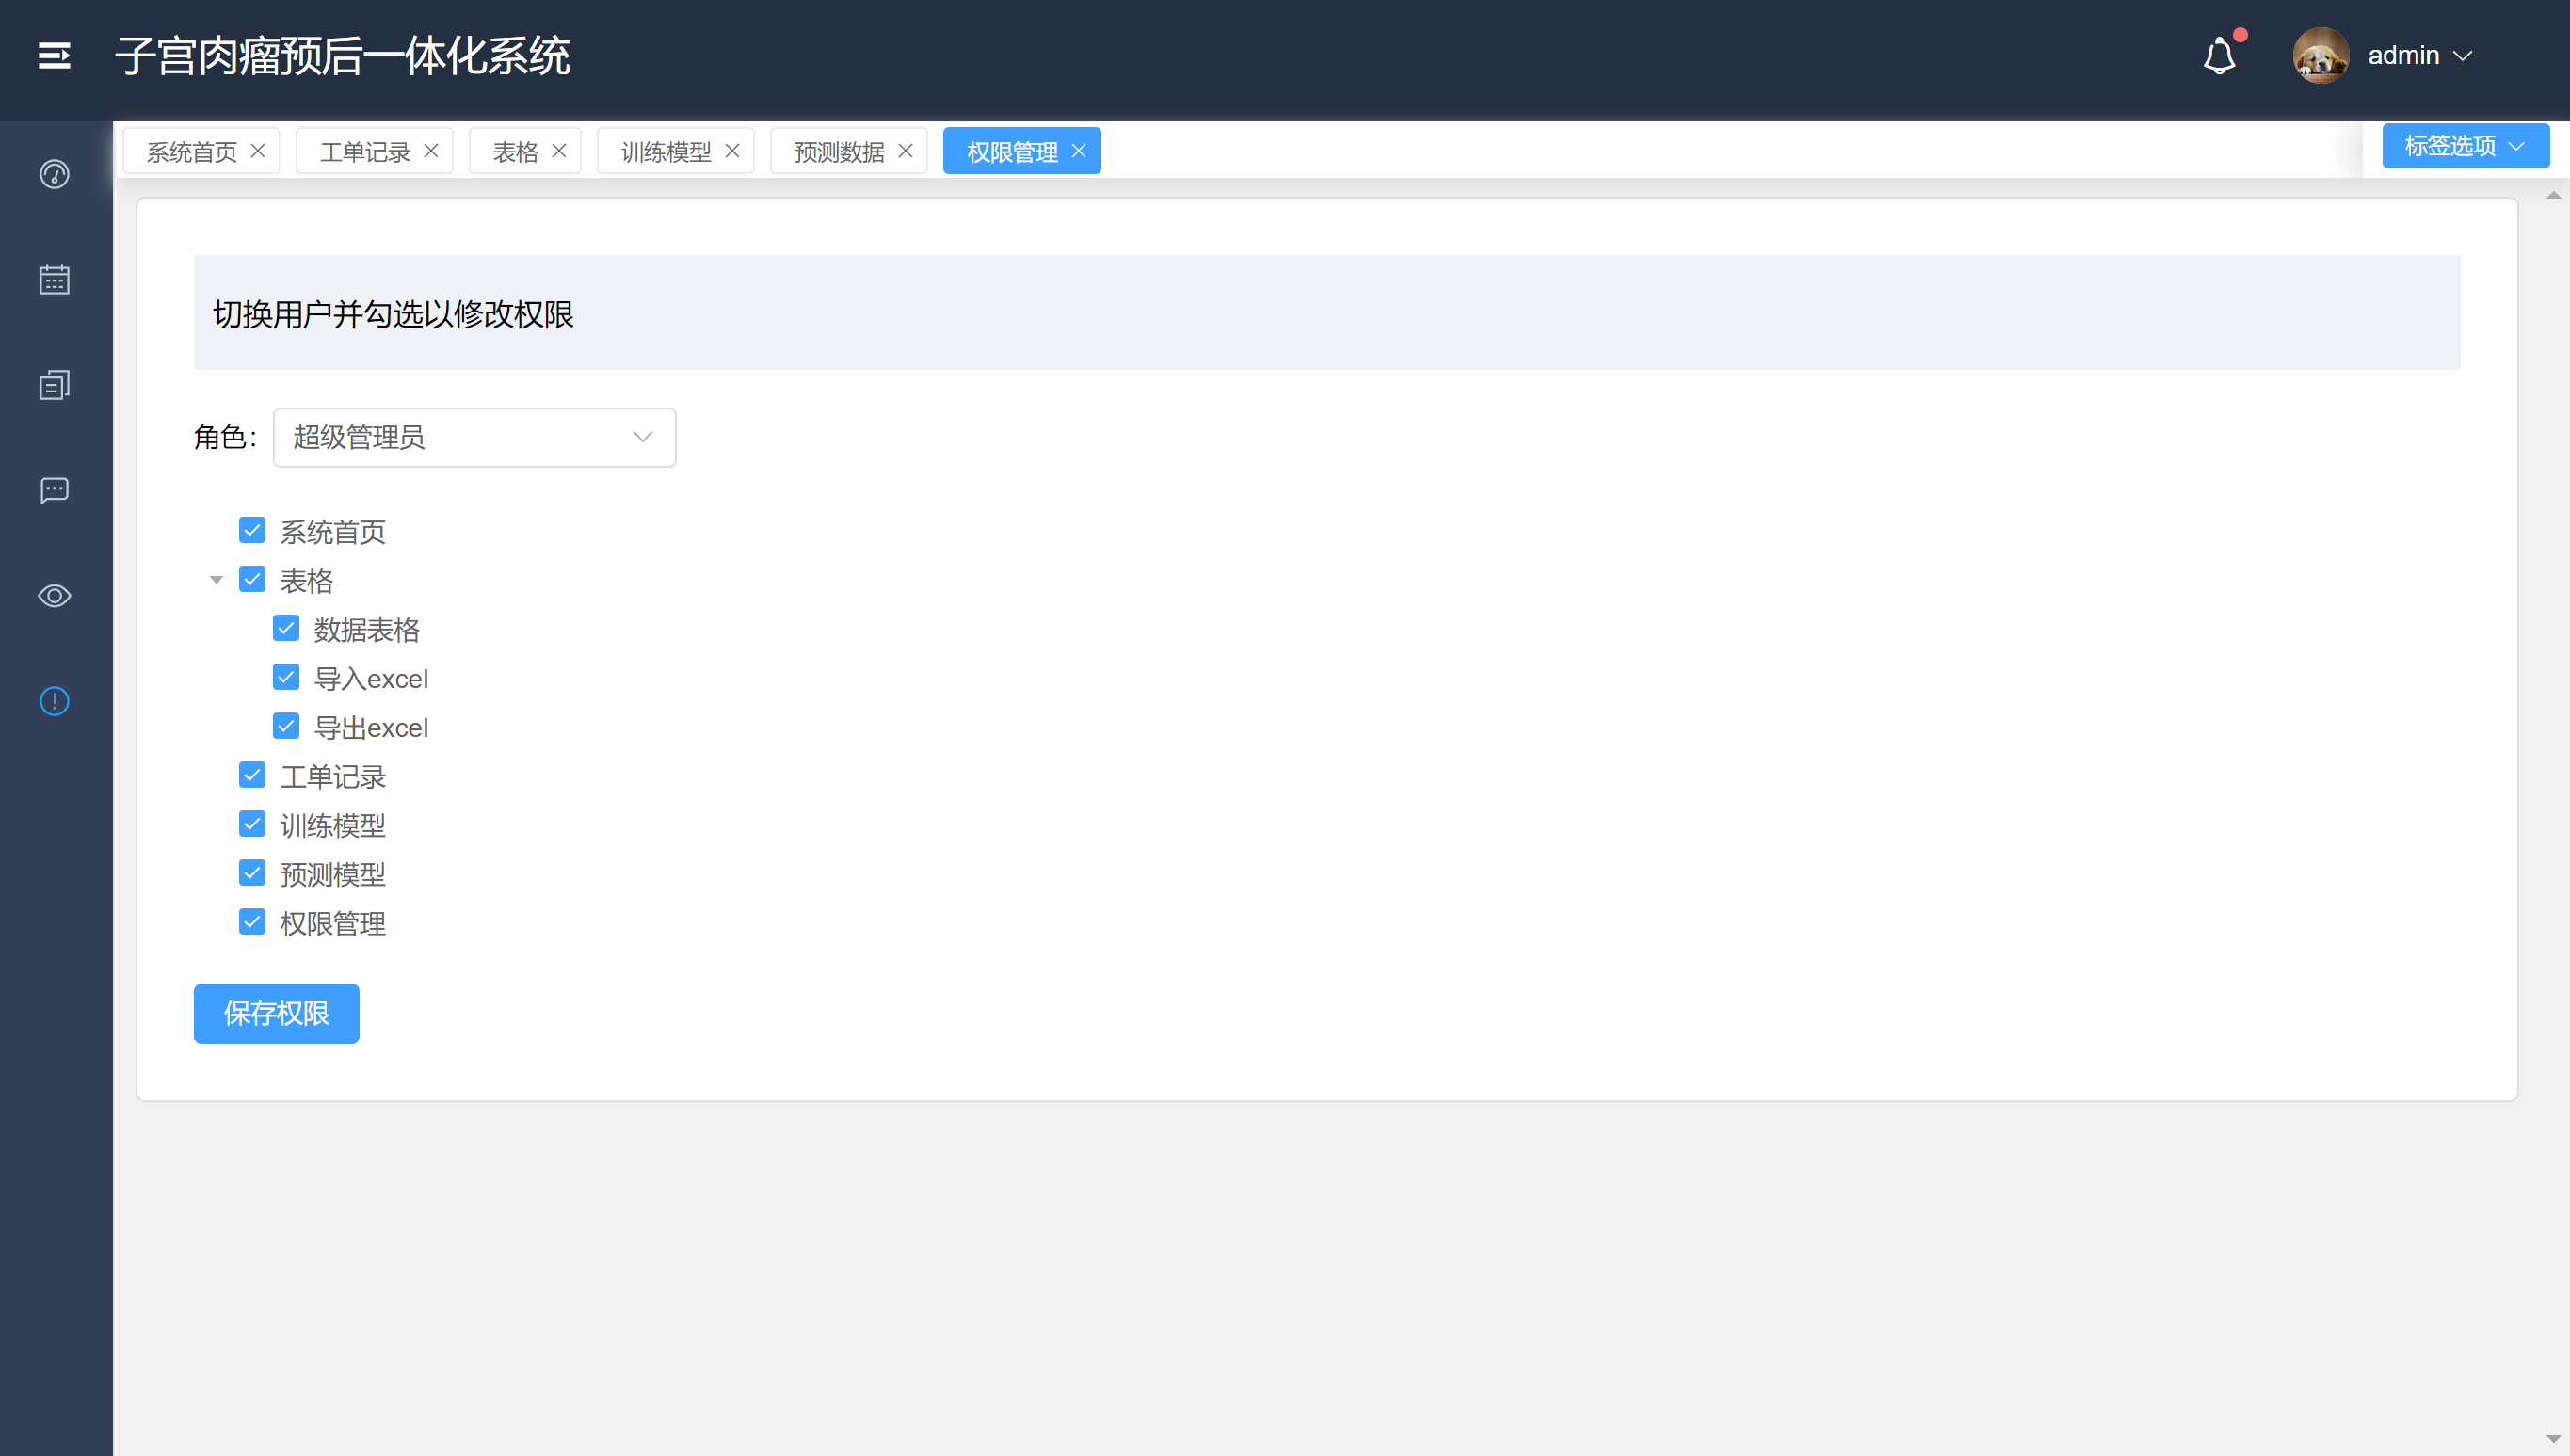
\includegraphics[scale=0.2]{page_pms.png}
    \caption{系统权限页面} \label{fig:page_pms}
\end{figure}